\documentclass{article}

\usepackage[utf8]{inputenc}
\usepackage[T1]{fontenc}
\usepackage{amsmath}
\usepackage{amssymb}
\usepackage{booktabs}
\usepackage{graphicx}
\usepackage{multirow}
\usepackage{xcolor}
\usepackage{url}
\usepackage{hyperref}
\usepackage[capitalize]{cleveref}
\usepackage{microtype}
\usepackage{geometry}
\geometry{margin=1in}

\title{Latent Bridge Matching for Fast Multi-Style Artistic Transfer}
\author{Anonymous Authors}
\date{}

\begin{document}
\maketitle

\begin{abstract}
Fast artistic style transfer remains difficult because style strength, content preservation, and computational efficiency often conflict. We study domain-level multi-style artistic transfer and propose a latent bridge-inspired framework that transports compact VAE latents with a style-conditioned velocity field. The method combines terminal sliced-Wasserstein distribution matching, which drives the endpoint toward the target artistic domain, with kinetic regularization, which penalizes excessive latent displacement and preserves content structure. A learnable style spatial prior and semantic cross-attention provide efficient domain-level style conditioning without per-image optimization or diffusion sampling. Under a strict 750-output protocol over five domains, the proposed model reaches a competitive raw CLIP-style score of 0.7161 while improving LPIPS-content over SaMST and substantially improving artifact-sensitive perceptual diagnostics including MUSIQ, MANIQA, DISTS-content, high-frequency patch KID, FFT slope error, and shallow Gram statistics. Destructive ablations show that terminal SWD is the primary style driver, kinetic regularization is essential for content preservation, and strong color matching damages the style-content trade-off. The results support a conservative but practically useful claim: latent bridge matching provides a clean, efficient, and reproducible style-content trade-off for fast multi-style artistic transfer.
\end{abstract}

\section{Introduction}
Artistic style transfer has long served as a testbed for separating image content from visual appearance. Classical neural style transfer showed that convolutional features and Gram statistics can synthesize compelling artistic textures \cite{gatys2016image}, while feed-forward arbitrary style transfer made real-time deployment practical through normalization-based style modulation \cite{huang2017adain}. More recent attention, transformer, training-free, and diffusion-based systems have improved flexibility and style fidelity \cite{park2019sanet,deng2022stytr2,hong2023aespa,huang2024aesfa,gim2024cast,chung2024styleid}. However, practical multi-style artistic transfer still exposes a persistent three-way tension: strong target-style expression, faithful content preservation, and low computational cost.

This tension is especially visible in domain-level multi-style transfer. Efficient multi-style systems can support many styles and fast inference, but the output may become washed, over-smoothed, or contaminated by structured grain artifacts. Diffusion-based or training-free methods can produce strong style semantics, but may be expensive or suffer semantic drift under content-preserving evaluation. In our local strict-750 protocol, for example, StyleID obtains the highest raw CLIP-style score but exhibits severe content collapse, while SaMST obtains strong raw style and content scores but produces visible muddy and grain-like texture artifacts. These observations suggest that standard style/content metrics alone are insufficient: a competitive system must also be evaluated for perceptual quality and artifact-sensitive texture realism.

We propose a fast latent-space multi-style artistic transfer framework that models stylization as a style-conditioned latent probability flow. Instead of directly predicting RGB images, the method transports a compact VAE latent through a neural velocity field. A terminal sliced-Wasserstein distance (SWD) term aligns generated endpoints with the target artistic domain, while kinetic regularization penalizes excessive latent displacement and preserves content. A learnable style spatial prior and semantic cross-attention provide a lightweight approximation to local style transport without per-image optimization or diffusion sampling.

Our contributions are:
\begin{itemize}
    \item We formulate domain-level multi-style artistic transfer as a bridge-inspired latent transport problem with separate terminal style matching and path-energy content preservation.
    \item We introduce an efficient style spatial prior and semantic cross-attention architecture that supports fast style-conditioned latent velocity prediction.
    \item We provide a strict 750-output evaluation protocol with complete local comparisons to AdaIN, S2WAT, SaMST, StyleID, and our method, together with artifact-sensitive diagnostics for grain and perceptual quality.
    \item We conduct destructive ablations and 40-run category-weight sweeps showing that terminal SWD drives style, kinetic regularization preserves content, and naive color matching harms the style-content trade-off.
\end{itemize}

\section{Related Work}
\paragraph{Classical and arbitrary neural style transfer.}
Neural style transfer began with optimization-based feature reconstruction and Gram-matrix style losses \cite{gatys2016image}. AdaIN later enabled real-time arbitrary transfer by aligning channel-wise feature statistics \cite{huang2017adain}. Attention-based methods such as SANet improved local style matching through style-attentional feature aggregation \cite{park2019sanet}. Recent aesthetic and pattern-aware methods, including AesPA-Net and AesFA, further emphasize pattern repeatability, aesthetic features, and high-quality arbitrary stylization \cite{hong2023aespa,huang2024aesfa}. These methods demonstrate the value of feature statistics and local matching, but they generally do not explicitly model a style-conditioned transport path with a terminal distribution constraint.

\paragraph{Transformer and multi-style transfer.}
Transformer-based style transfer methods such as StyTr2 and S2WAT use attention mechanisms to improve content-style interaction and long-range feature modeling \cite{deng2022stytr2,xia2024s2wat}. Multi-style approaches aim to amortize many styles in a single compact system; SaMST is a recent representative emphasizing pluggable style representations, low parameter count, and fast inference \cite{liu2024samst}. These systems are directly related to our goal of efficient multi-style transfer. In contrast to representation-only style injection, our method embeds semantic cross-attention inside a latent bridge objective, allowing terminal distribution matching and kinetic regularization to explicitly shape the style-content trade-off.

\paragraph{Training-free and diffusion-based style transfer.}
Training-free and diffusion-based approaches provide a different route to flexible style transfer. CAST uses VQ autoencoders for content-adaptive training-free style transfer \cite{gim2024cast}, while StyleID injects style into large-scale diffusion models without training \cite{chung2024styleid}. These methods can be visually strong, but diffusion sampling and semantic drift can limit their suitability for fast domain-level transfer. Our work targets a complementary efficiency regime: compact latent integration with style-id conditioning rather than iterative diffusion sampling or per-style optimization.

\paragraph{Distribution matching and perceptual evaluation.}
Our objective is motivated by optimal transport and distribution matching. Sinkhorn distances and computational optimal transport provide efficient tools for approximate transport problems \cite{cuturi2013sinkhorn,peyre2019computational}, while the Schrodinger problem connects entropic transport to stochastic path measures \cite{leonard2014survey}. We use SWD as a lightweight terminal distribution matching objective. For evaluation, we combine perceptual and distributional measures including LPIPS \cite{zhang2018lpips}, FID \cite{heusel2017fid}, KID \cite{binkowski2018kid}, DISTS \cite{ding2020dists}, MUSIQ \cite{ke2021musiq}, MANIQA \cite{yang2022maniqa}, and style-transfer-specific ArtFID \cite{wright2022artfid}. This broad metric set is important because raw CLIP-style and structural scores may fail to penalize grain-like artifacts.

\section{Method}
\subsection{Latent bridge formulation}
Let $z_0 \in \mathbb{R}^{4 \times 32 \times 32}$ denote the VAE latent of a content image and let $s$ denote a target style/domain identifier. The model learns a style-conditioned velocity field
\begin{equation}
    v_\theta(z_t,t,s),
\end{equation}
which transports content latents toward the target artistic domain. At inference time, the endpoint is obtained with explicit Euler integration:
\begin{equation}
    z_{t+\Delta t} = z_t + v_\theta(z_t,t,s)\Delta t .
\end{equation}
The primary evaluation uses 12 integration steps and step size 1.0. We interpret this as a bridge-inspired latent probability flow rather than a strict solver for the continuous-time Schrodinger Bridge problem. The formulation is nevertheless useful: terminal distribution matching controls where the trajectory ends, while path-energy regularization controls how far it moves from the content latent.

\subsection{Architecture}
The implementation uses \texttt{TimeConditionedLANCETBridge(LatentAdaCUT)}. The backbone lifts the $4$-channel latent to 128 channels, processes high-resolution $32 \times 32$ features, downsamples to a $16 \times 16$ body representation, applies four semantic cross-attention/body blocks, upsamples, fuses skip features, and decodes a latent velocity. The target style is represented by a learnable spatial prior
\begin{equation}
    P_s \in \mathbb{R}^{C \times 16 \times 16},
\end{equation}
where $s$ ranges over \{photo, Hayao, Monet, Van Gogh, Cezanne\}. This style prior is a domain-level prototype rather than a per-reference image representation. It enables fast inference but also limits raw reference-specific style capacity.

Semantic cross-attention injects the style prior into content features:
\begin{equation}
    Q=f_c(x), \quad K,V=f_s(P_s), \quad A=\operatorname{softmax}(QK^\top/\tau), \quad \hat{x}=AV .
\end{equation}
The primary model uses semantic attention temperature 0.12, style attention temperature 0.08, and style attention sharpen scale 2.5. Skip fusion uses an additive projected route to preserve spatial content structure.

\subsection{Training objective}
Training uses an OMF-style endpoint approximation. For a content latent $z_0$ and target style $s$, the model predicts a velocity at the endpoint training time and forms
\begin{equation}
    \hat{z}_1 = z_0 + v_\theta(z_0,1,s).
\end{equation}
The loss combines kinetic regularization and terminal SWD:
\begin{equation}
    \mathcal{L} = \lambda_{\mathrm{kin}}\mathcal{L}_{\mathrm{kin}} + \lambda_{\mathrm{swd}}\mathcal{L}_{\mathrm{swd}}.
\end{equation}
The kinetic term is
\begin{equation}
    \mathcal{L}_{\mathrm{kin}} = \mathbb{E}\|v_\theta(z_0,1,s)\|_2^2,
\end{equation}
which penalizes excessive latent displacement. The terminal SWD term compares generated endpoint patches with target-style patches over 64 sliced projections and patch sizes 3, 5, 7, and 15. The primary configuration uses $\lambda_{\mathrm{kin}}=1.0$ and $\lambda_{\mathrm{swd}}=20.0$. Color, cycle, NCE, and repulsive losses are disabled in the main setting. This separation between endpoint style distribution matching and path-energy regularization is the central mechanism behind the observed style-content Pareto behavior.

\begin{figure}[t]
    \centering
    
\includegraphics[width=0.95\linewidth]{../figures/fig_framework_overview.png}
    \caption{Overview of the proposed latent bridge-inspired style transfer framework. A content image is encoded into a compact latent, transported by a style-conditioned velocity field, constrained by terminal SWD and kinetic regularization, and decoded into a stylized output.}
    \label{fig:framework}
\end{figure}

\section{Experiments}
\subsection{Protocol and metrics}
We evaluate under a strict 750-output protocol: five source domains times five target domains times 30 source images. The five domains are photo, Hayao, Monet, Van Gogh, and Cezanne; Ukiyo-e is not used in the present protocol. We report CLIP-style, CLIP-content, LPIPS-content, and the composite score
\begin{equation}
    \mathrm{EC} = \mathrm{CLIP\mbox{-}style}\cdot(1-\mathrm{LPIPS}).
\end{equation}
For artifact-sensitive analysis we also report MUSIQ, MANIQA, DISTS-content, high-frequency patch KID, FFT slope error, and shallow Gram micro statistics. Complete strict-750 local outputs are available for Ours, SaMST, StyleID, S2WAT, and AdaIN variants.

\subsection{Main comparison}
\begin{table*}[t]
\centering
\caption{Strict-750 comparison. Higher is better for CLIP-S, CLIP-C, EC, MUSIQ, and MANIQA. Lower is better for LPIPS, DISTS, HF-KID, and KID.}
\label{tab:main}
\begin{tabular}{lrrrrrrrrr}
\toprule
Method & CLIP-S & CLIP-C & LPIPS & EC & MUSIQ & MANIQA & DISTS & HF-KID & KID \\
\midrule
Ours K1 epoch 7 & 0.7161 & 0.8086 & 0.4514 & 0.3928 & 49.2059 & 0.4057 & 0.2477 & 4.1694 & 0.0524 \\
Ours K1 epoch 8 & 0.7167 & 0.7977 & 0.4615 & 0.3859 & -- & -- & -- & -- & 0.0554 \\
SaMST strict & 0.7194 & 0.8193 & 0.4664 & 0.3839 & 36.0950 & 0.3139 & 0.2943 & 6.7598 & 0.0489 \\
StyleID strict & 0.7597 & 0.5519 & 0.7497 & 0.1902 & -- & -- & -- & -- & -- \\
S2WAT strict & 0.7139 & 0.7465 & 0.5263 & 0.3382 & 36.5256 & 0.1754 & 0.2942 & 12.6623 & 0.0567 \\
AdaIN v32k & 0.7130 & 0.6990 & 0.6298 & 0.2639 & -- & -- & -- & -- & -- \\
AdaIN vgg19 & 0.6930 & 0.5991 & 0.6870 & 0.2169 & -- & -- & -- & -- & -- \\
\bottomrule
\end{tabular}
\end{table*}

Table~\ref{tab:main} shows that Ours epoch 7 is close to SaMST in raw CLIP-style while improving LPIPS and EC. StyleID obtains the highest CLIP-style, but its CLIP-content of 0.5519 and LPIPS of 0.7497 indicate severe semantic drift. AdaIN variants are substantially weaker in content preservation. S2WAT reaches a comparable style score but has worse LPIPS and much worse HF-Patch-KID.

\begin{figure}[t]
    \centering
    
\includegraphics[width=0.82\linewidth]{../figures/fig_quality_tradeoff.png}
    \caption{Strict-750 style-content trade-off. Ours is close to SaMST in raw CLIP-style while retaining a better LPIPS-based trade-off than several baselines; StyleID reaches high style but collapses content.}
    \label{fig:tradeoff}
\end{figure}

\subsection{Artifact-sensitive comparison to SaMST}
SaMST is a strong baseline under raw style and structure metrics, but visual inspection revealed muddy and grain-like artifacts. We therefore examine artifact-sensitive diagnostics in Table~\ref{tab:artifact}. Ours improves MUSIQ by 13.1109, MANIQA by 0.0918, DISTS-content by 0.0466, HF-Patch-KID by 2.5904, and FFT slope error by 0.5063. These results support the interpretation that SaMST preserves low-frequency structure but produces less realistic local texture statistics.

\begin{table}[t]
\centering
\caption{Artifact-sensitive comparison between Ours and SaMST.}
\label{tab:artifact}
\begin{tabular}{lrr}
\toprule
Metric & Ours e7 & SaMST \\
\midrule
MUSIQ $\uparrow$ & 49.2059 & 36.0950 \\
MANIQA $\uparrow$ & 0.4057 & 0.3139 \\
DISTS-content $\downarrow$ & 0.2477 & 0.2943 \\
HF-Patch-KID $\downarrow$ & 4.1694 & 6.7598 \\
FFT slope error $\downarrow$ & 0.5473 & 1.0536 \\
Gram micro $\downarrow$ & 0.0798 & 0.0947 \\
\bottomrule
\end{tabular}
\end{table}

\begin{figure}[t]
    \centering
    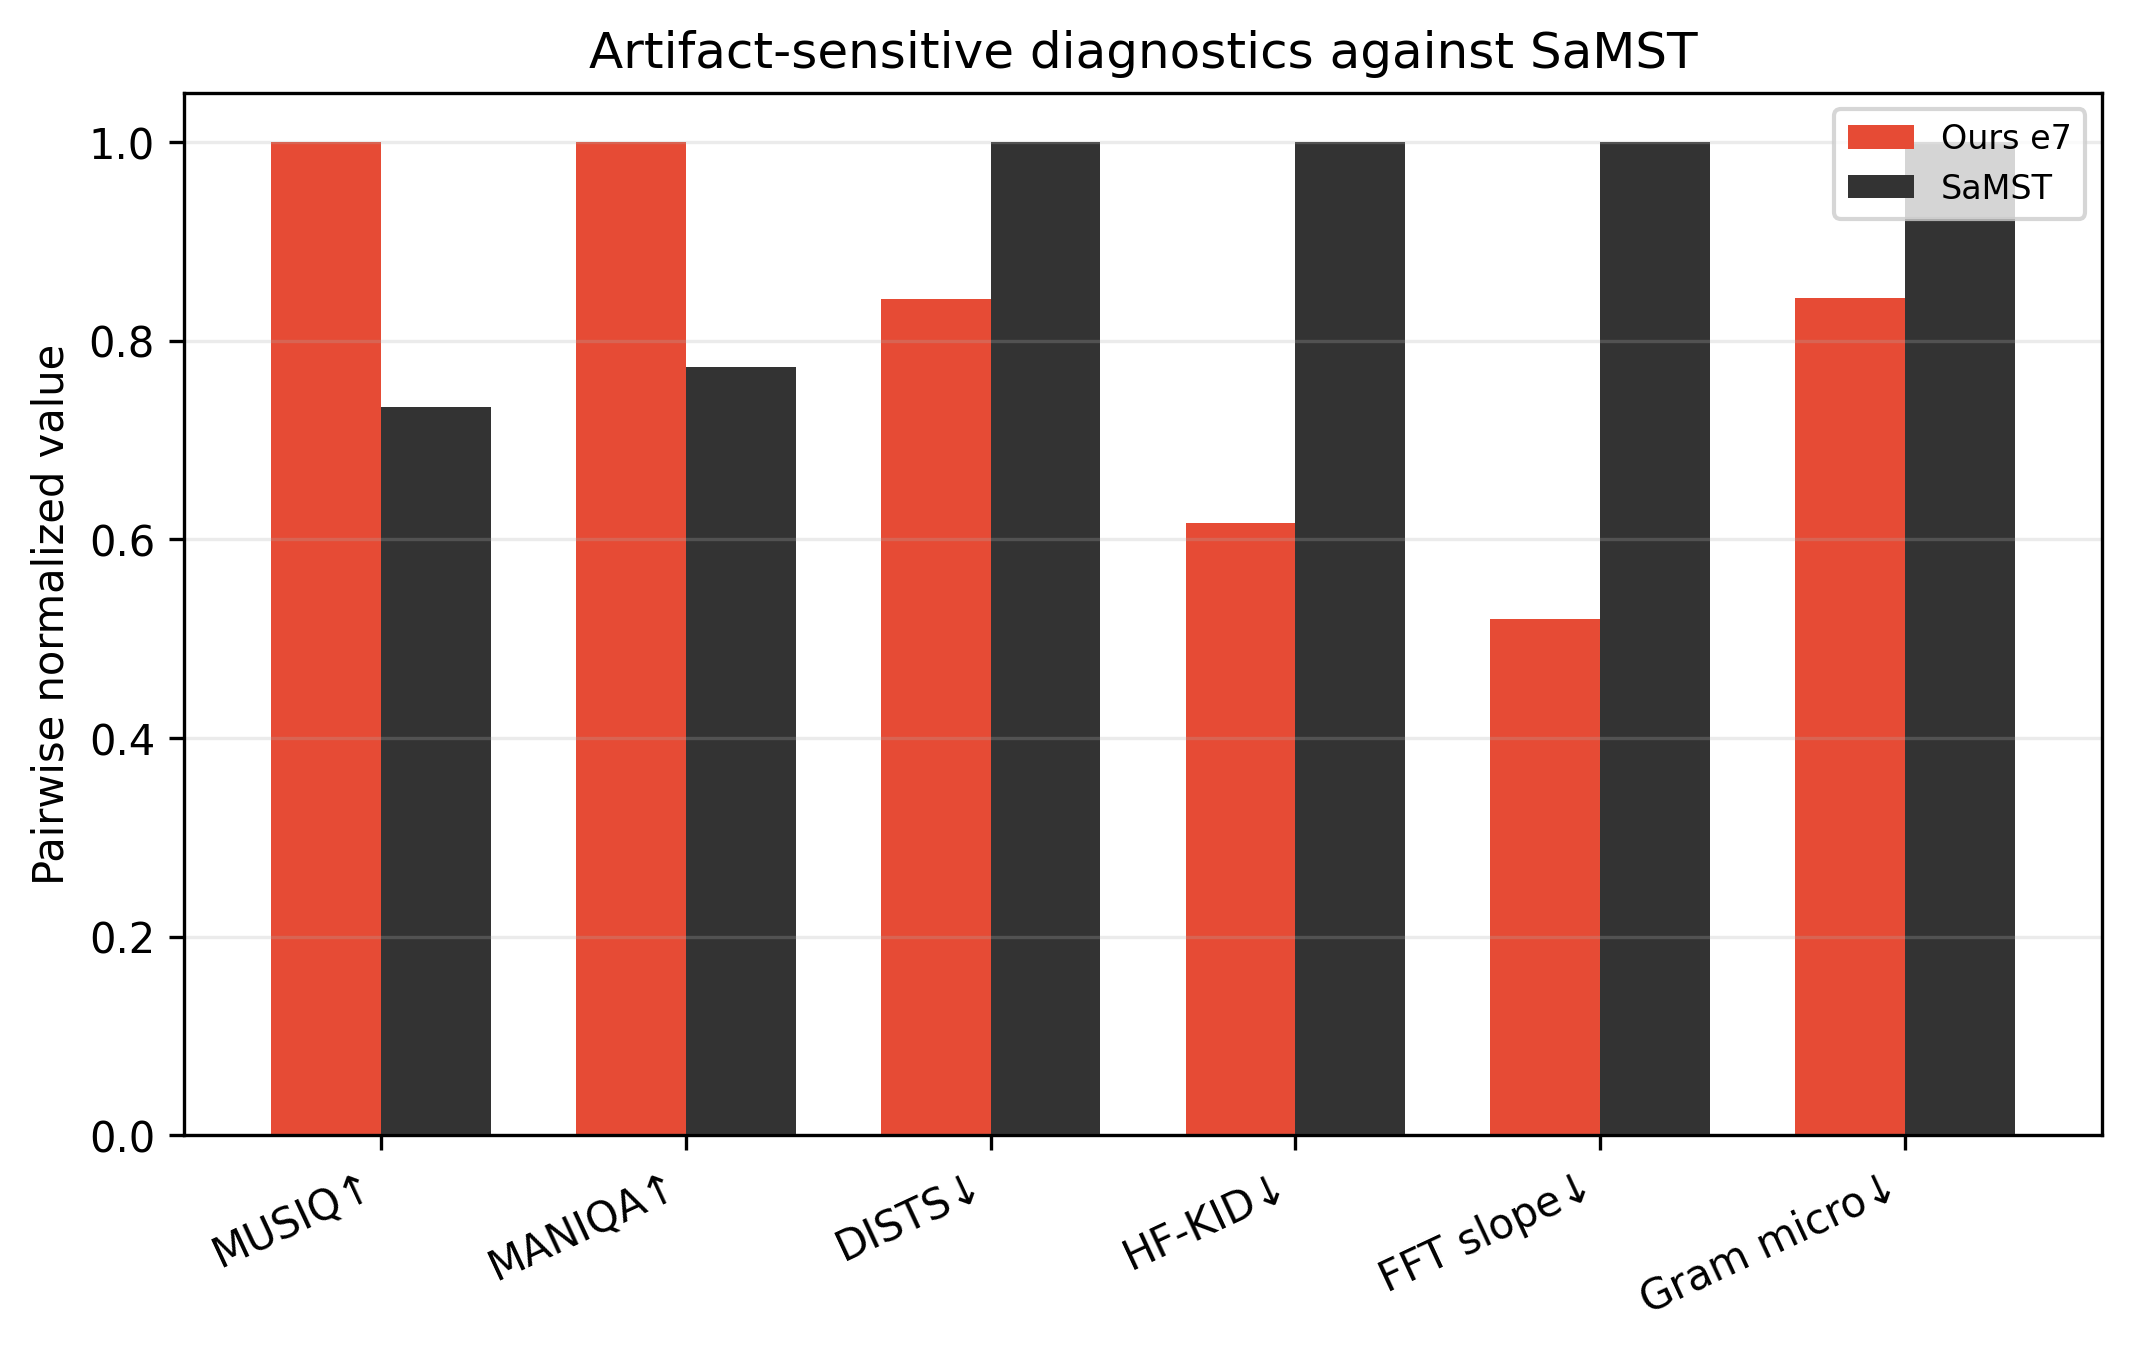
\includegraphics[width=0.86\linewidth]{../figures/fig_artifact_diagnostics.png}
    \caption{Artifact-sensitive diagnostics for Ours and SaMST. Mixed-scale metrics are pairwise normalized for readability; the raw numeric values are reported in the experimental table.}
    \label{fig:artifact}
\end{figure}

\subsection{Destructive ablations}
\begin{table}[t]
\centering
\caption{Destructive ablations under the strict-750 protocol.}
\label{tab:ablation}
\begin{tabular}{lrrrr}
\toprule
Variant & CLIP-S & CLIP-C & LPIPS & EC \\
\midrule
D0 full & 0.7014 & 0.8022 & 0.4593 & 0.3791 \\
D1 w/o terminal SWD & 0.6708 & 0.8989 & 0.3490 & 0.4368 \\
D2 w/o kinetic & 0.7159 & 0.6624 & 0.6375 & 0.2596 \\
D8 strong color loss & 0.6923 & 0.6629 & 0.5675 & 0.2994 \\
\bottomrule
\end{tabular}
\end{table}

The ablation results in Table~\ref{tab:ablation} expose the mechanism of the model. Removing terminal SWD gives excellent content preservation but weak style, showing that terminal distribution matching is the primary style driver. Removing kinetic regularization preserves style but collapses content, confirming that the path-energy penalty is essential. Strong color loss damages both content and distributional quality, so naive color matching is not used in the mainline.

\begin{figure}[t]
    \centering
    
\includegraphics[width=0.82\linewidth]{../figures/fig_ablation_pareto.png}
    \caption{Destructive ablations. Removing terminal SWD improves content but weakens style, while removing kinetic regularization increases style at the cost of severe content degradation.}
    \label{fig:ablation}
\end{figure}

\subsection{Weight sweep and theory switches}
The 40-run category-weight sweep trained 20 sampling recipes with $K \in \{1,2\}$ for eight epochs each, evaluating every epoch for 320 total checkpoints. The best EC result was K2 balanced default at epoch 3 with CLIP-style 0.6980, CLIP-content 0.8727, LPIPS 0.3777, and EC 0.4343. The best raw-style result in the sweep was K1 balanced default at epoch 8 with CLIP-style 0.7161, CLIP-content 0.7984, LPIPS 0.4605, and EC 0.3863. The sweep showed that more complex category weighting was not consistently better than balanced sampling.

\begin{figure}[t]
    \centering
    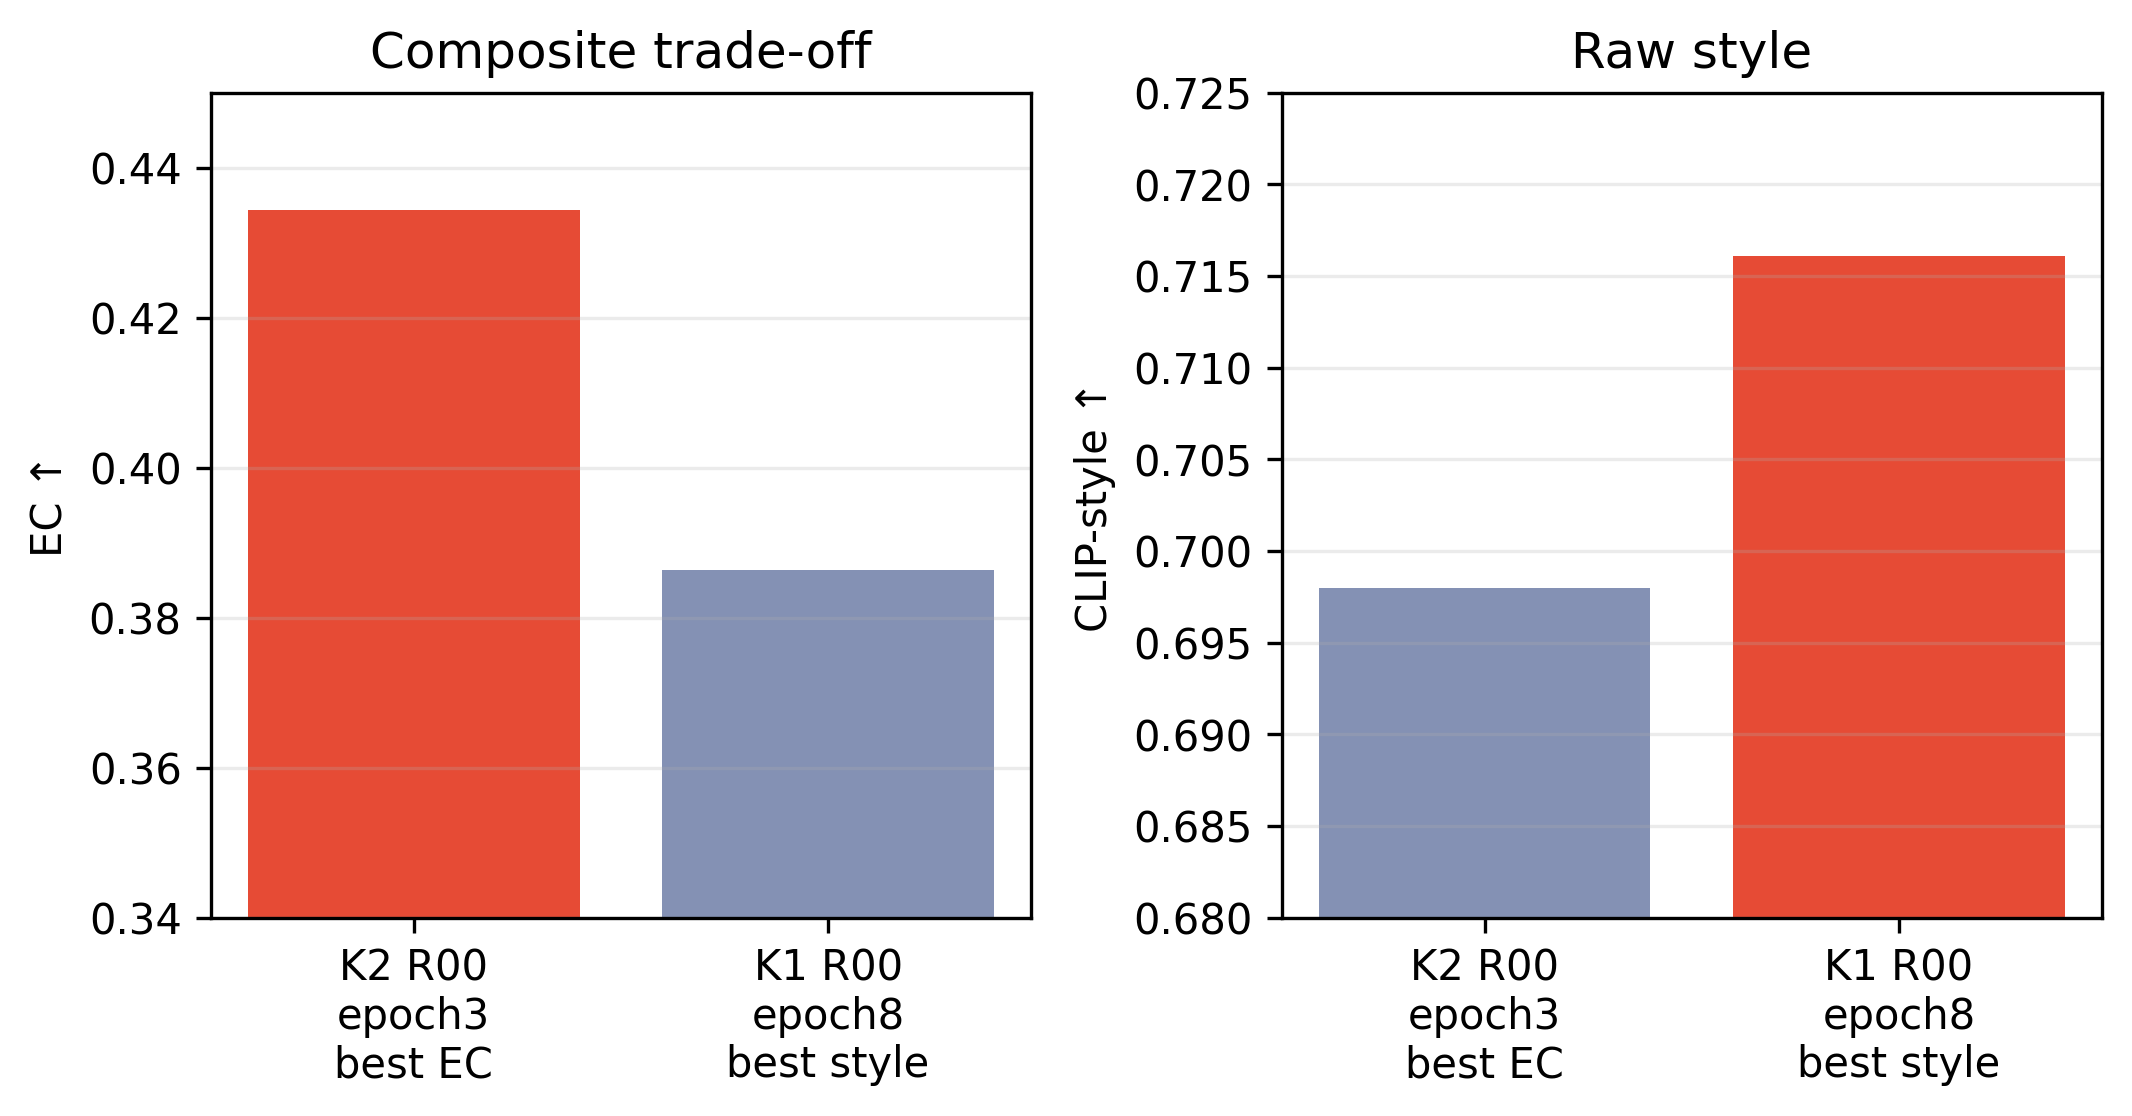
\includegraphics[width=0.86\linewidth]{../figures/fig_weight_sweep_summary.png}
    \caption{Summary of the 40-run category-weight sweep. K2 balanced default gives the best EC, whereas K1 balanced default gives the best raw CLIP-style among evaluated checkpoints.}
    \label{fig:sweep}
\end{figure}

We also evaluated optional theory switches. Sinkhorn-normalized semantic routing and entropy-gated kinetic regularization improved EC/content but reduced raw CLIP-style. The best theory-switch EC was entropy-gated kinetic with weight 5.0 at epoch 1, giving CLIP-style 0.6916, CLIP-content 0.8804, LPIPS 0.3684, and EC 0.4368. Color transport increased raw style slightly but harmed LPIPS and content, and was therefore not selected as the mainline.

\section{Discussion and Limitations}
The experiments support a specific and conservative conclusion. The proposed method does not universally dominate all baselines on raw style: StyleID has higher CLIP-style, and SaMST is slightly higher than Ours epoch 7 on raw CLIP-style and CLIP-content. However, StyleID suffers content collapse, while SaMST exhibits grain-like artifacts that are poorly captured by standard structure metrics. Ours provides a cleaner style-content trade-off and stronger artifact-sensitive perceptual quality under the local strict-750 protocol.

The current study has several limitations. Complete strict-750 runs are not yet available for CAST, AesFA, AesPA-Net, and StyTr2, so they should not be over-discussed as fully matched baselines. User-study data has not yet been collected, which is important for validating perceptual cleanliness and artifact preference. Finally, the style representation is domain-level rather than reference-image-specific; this makes inference efficient but limits the ability to reproduce unique single-image brushstroke patterns. Future work should evaluate controlled integration horizons, semantic paint gains, K schedules, richer domain prototype priors, high-resolution generalization, and human preference studies.

\section{Conclusion}
We presented a latent bridge-inspired framework for fast multi-style artistic transfer. By combining terminal SWD style distribution matching with kinetic path regularization, the method separates the forces that drive style from those that preserve content. A lightweight style spatial prior and semantic cross-attention make this formulation practical for efficient domain-level transfer. Under a strict 750-output evaluation, the method reaches a competitive raw style score while improving LPIPS and artifact-sensitive perceptual diagnostics over SaMST and preserving content substantially better than StyleID. The results indicate that latent bridge matching is a promising foundation for fast, clean, and reproducible artistic style transfer.

\clearpage
\bibliographystyle{plain}
\bibliography{refs}

\end{document}

